\section{CortexDecoder}
\label{sec:cortex_decoder}
CortexDecoder is a two-branch brain decoding framework that maps cortical flatmap representations to high-level semantic and low-level visual features for image reconstruction. The model first encodes cortical flatmaps using a pretrained CortexMAE encoder, producing spatially organized brain tokens. These brain tokens are then fed into the cross-attention bridge, which predicts visual image features. The semantic branch predicts unpooled CLIP embeddings, while the low-level branch predicts VGG features. Finally, the predicted visual representations are provided to a frozen diffusion decoder to reconstruct the corresponding image.

All model training and evaluations were performed on a single NVIDIA H100 GPU (80 GB). Both branches were trained separately with AdamW \cite{loshchilov2019decoupledweightdecayregularization} (learning rate 5e-4, weight decay 1e-2) and a batch size of 128 under bfloat16 mixed precision. Both the semantic branch and the low-level branch were trained for 25 epochs. Deep Image Prior inversion at inference uses 2,000 Adam steps per image with 36 images optimized in parallel on the GPU.

\subsection{Natural Scenes Dataset}

The Natural Scenes Dataset (NSD) is a large-scale 7T fMRI dataset in which eight participants viewed natural images drawn from MS-COCO (Microsoft Common Objects in Context) \cite{lin2015microsoftcococommonobjects} across up to 40 scan sessions each. Each session comprises 750 trials; in each trial, one image is presented for 3 seconds, followed by a 1-second blank. Each subject viewed 10,000 unique images, each repeated 3 times, for a total of 30,000 trials per subject. A subset of 1000 images (shared1000) was presented to all subjects and is reserved as a standard test set throughout the literature.
The NSD experiment uses a rapid event-related design in which a new image stimulus is presented every 4 seconds, so successive stimuli occur within the timescale of the hemodynamic response. Because the responses to successive trials overlap, single-trial responses cannot be read directly from the time series. A general linear model (GLM) \cite{10.7554/eLife.77599} performs this deconvolution, and its output is a static spatial map of cortical activity per trial rather than a time series. This is precisely the form that 2D flatmap representations and patch-based tokenization assume. We note that the CortexMAE encoder is spatiotemporal and retains a temporal patch dimension from its pretraining on the BOLD time series. However, because our inputs are static single-trial beta maps, we do not utilize this temporal dimension in CortexDecoder.

\subsection{MAE Encoder and Tokenization}
NSD’s surface betas are distributed on a fsaverage mesh \cite{FISCHL2012774} (163,842 vertices per hemisphere). We resample them to fsLR-32k (32,492 vertices per hemisphere, 64,984 total), the standard HCP (Human Connectome Project) \cite{VanEssen_Smith_Barch_Behrens_Yacoub_Ugurbil_2013} mesh on which CortexMAE was pretrained. A pycortex-based \cite{DBLP:journals/fini/GaoHLG15} flat-surface resampler then projects these vertices onto a single-channel $224\times560$ raster, producing the 2D cortical flatmap. Since the projection is defined by a common template mesh rather than by individual anatomy, a given location in the raster corresponds to approximately the same piece of cortex across subjects.
The flatmap is divided into non-overlapping $16\times16$ spatial patches, forming a $14\times35$ grid of 490 cells. Since the cortical surface occupies only part of the bounding box, 364 cells contain cortex and the remaining cells are background. CortexMAE uses a validity mask to exclude these background patches, so only 364 cortical patches are embedded.
CortexMAE is a spatiotemporal masked autoencoder \cite{he2021maskedautoencodersscalablevision} pretrained on BOLD time series. In other words, its patch embedding operates over both space and time. In our case, the input is a single-trial beta map, which has no temporal component. To use the pretrained model, we represent each beta map as a static 16-frame clip. Since we use the CortexMAE encoder out of the box, we also retain its output shape, a sequence of 1456 tokens each with a dimension of 768.

\begin{figure}[!t]
\centering
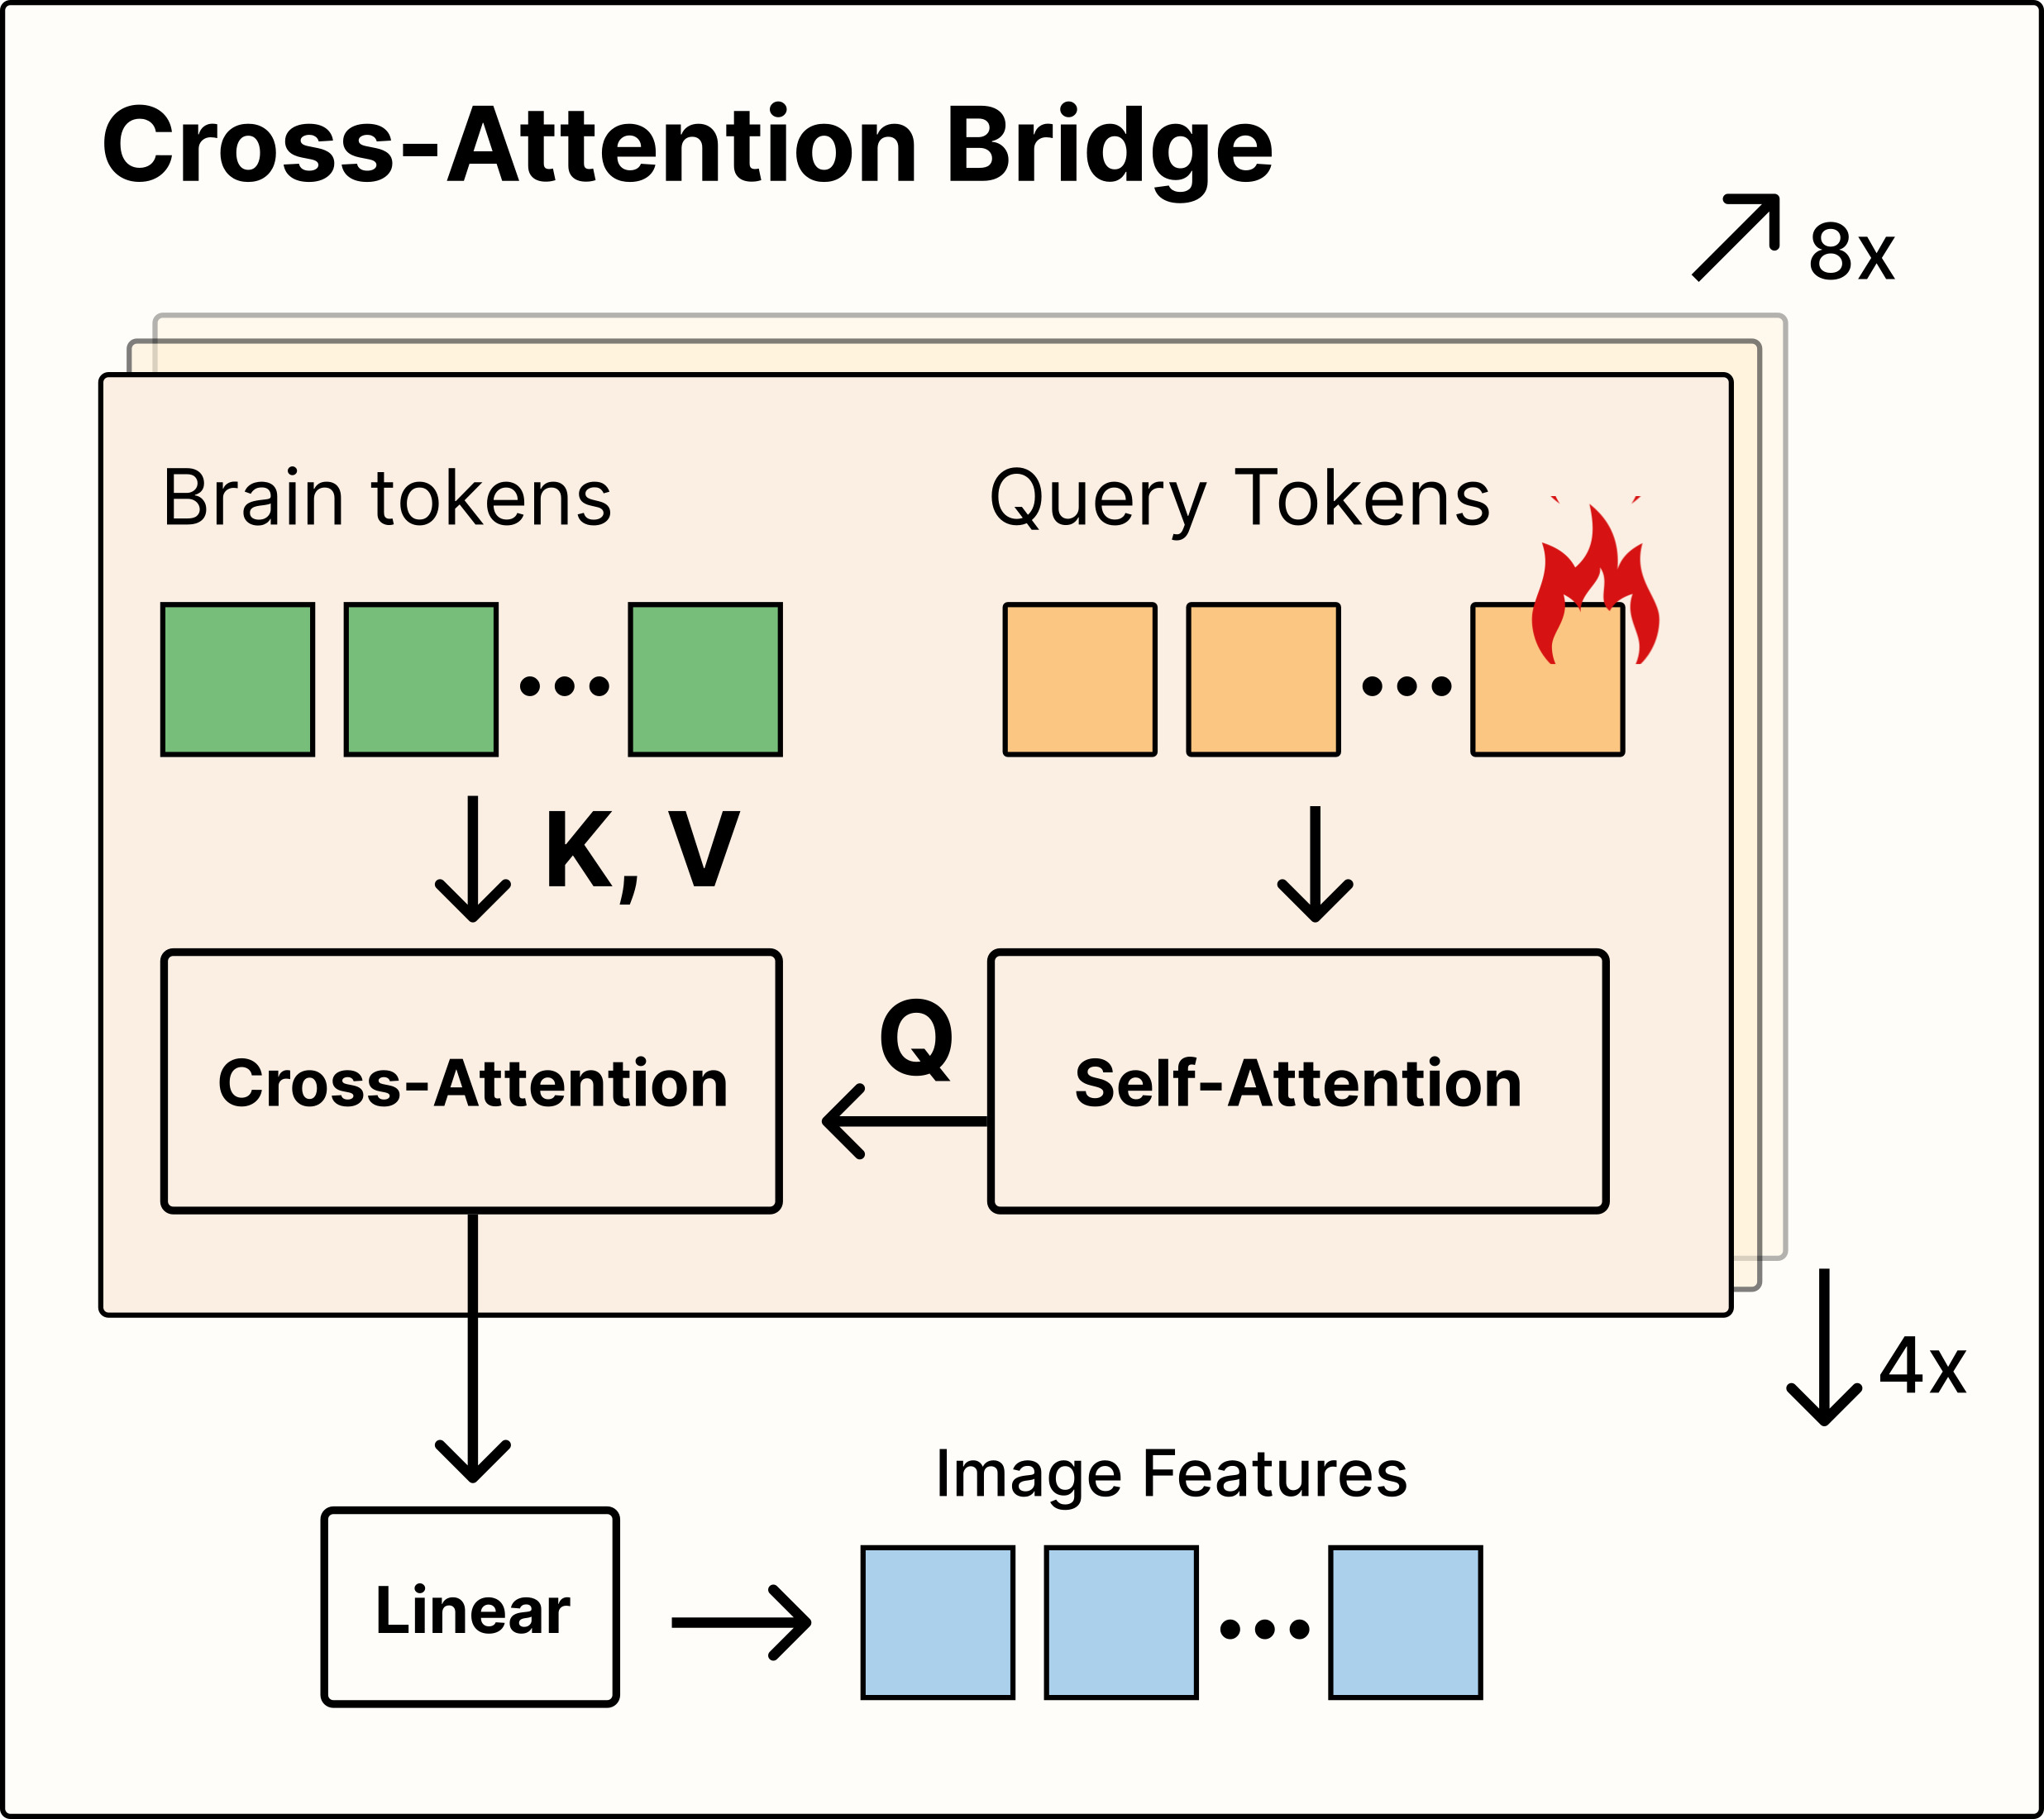
\includegraphics[width=0.8\columnwidth]{images/cross.jpg}
\caption{Cross-attention bridge. Learned queries, one per output token, attend to the brain tokens through 4 blocks of self-attention, cross-attention and FFN. A linear layer projects each query to the target feature dimension. Each branch has its own bridge. Images from COCO \cite{lin2015microsoftcococommonobjects} (CC BY 4.0).}
\label{fig:cross_attention_bridge}
\end{figure}

\subsection{Cross-Attention Bridge}
The bridge maps the sequence of brain tokens to a sequence of visual feature tokens. Its design follows DETR (DEtection TRansformer) \cite{DBLP:journals/corr/abs-2005-12872}. We define a set of learned query vectors with one query per output token. These are randomly initialized and trained jointly with the rest of the model. Each query is responsible for predicting one token of the target visual representation.
The brain tokens serve as memory. They are layer-normalized and projected to the model width when the two dimensions differ. In our case, the CortexMAE embedding dimension and the bridge width are both 768, so no projection is needed. The queries are then passed through a stack of transformer decoder layers. Each layer applies self-attention among the queries, then cross-attention from the queries into the brain memory, and finally a position-wise feed-forward network (FFN). Self-attention lets the queries coordinate with one another so that neighboring output tokens can share information. Cross-attention is where the decoding happens. Each query attends over all 1456 brain tokens and pools the ones that carry information about its target feature. A final linear layer projects each decoded query to the dimensionality of the target representation.
We use 4 decoder layers and 8 attention heads. The model width is 768, with a feed-forward dimension of 3072 and dropout of 0.1. The semantic and low-level branches share these settings.
The key property of this design is that the brain representation remains a sequence throughout the pipeline. Each query attends over the full set of brain tokens. A pooled brain vector would make every query attend to the same input and reduce the decoder to a multilayer perceptron (MLP) applied identically at each output position.

We instantiate the bridge twice with one instance per branch and train the two independently rather than sharing a trunk. The semantic branch uses 256 queries and projects to 1664 dimensions. This matches the shape of the unpooled OpenCLIP ViT-bigG/14 \cite{radford2021learningtransferablevisualmodels, ilharco_gabriel_2021_5143773, schuhmann2022laionb} patch tokens that the diffusion decoder expects as conditioning. The low-level branch uses 7190 queries and projects to 512 dimensions. This matches the concatenated token count of the five VGG16-BN feature layers described in \cref{sec:low_level}. The two branches therefore differ by more than an order of magnitude in output length. They also optimize different losses, since the semantic target is dense and continuous, while the low-level target is better matched by a contrastive objective.

\begin{equation}
\mathcal{L}_{\mathrm{CLIP}} = \mathrm{MSE}\big(\hat{\mathbf{C}}, \mathbf{C}\big),
\end{equation}

\medskip

where $\hat{\mathbf{C}}, \mathbf{C} \in \mathbb{R}^{256 \times 1664}$ are the predicted and target OpenCLIP token sequences, and the error is averaged over all tokens, dimensions and images in the batch.

To train the low-level branch, we extract target tokens from five intermediate layers of a frozen VGG16-BN network (\texttt{relu1\_2} through \texttt{relu5\_3}, totaling $7{,}190$ spatial tokens of dimension $D=512$). For memory efficiency during training, we randomly sub-sample $K\in \{512, 512, 128, 64, 16\}$ query positions per layer at each step and compute a symmetric position-wise InfoNCE contrastive loss across the mini-batch of $B$ trials:

\begin{equation}
\mathcal{L}_{\mathrm{VGG}} =
\frac{1}{2K}\sum_{k=1}^{K}\left[\mathrm{CE}\!\left({\scriptstyle
\frac{\hat{\mathbf{z}}_{:,k}\mathbf{z}_{:,k}^{\top}}{\tau}},
\mathbf{y}\right) + \mathrm{CE}\!\left({\scriptstyle \frac{\mathbf{z}_{:,
k}\hat{\mathbf{z}}_{:,k}^{\top}}{\tau}}, \mathbf{y}\right)\right],
\end{equation}
where $\hat{\mathbf{z}}_{:,k}, \mathbf{z}_{:,k} \in \mathbb{R}^{B \times
D}$ denote the $\ell_2$-normalized predicted and ground-truth feature
matrices at spatial token $k$, $\tau = 0.07$ is the temperature
hyperparameter, and $\mathbf{y} = (1, \dots, B)^{\top}$ indexes the
matching trial pairs across the batch. The final low-level objective
averages $\mathcal{L}_{\mathrm{VGG}}$ equally across all five VGG16-BN layers.

\subsection{Semantic Branch}
The semantic branch predicts the image representations that condition the diffusion decoder. Its target is the unpooled patch-token sequence produced by the OpenCLIP ViT-bigG/14 vision encoder pretrained on LAION-2B \cite{schuhmann2022laionb}. For each stimulus image, we take the 256 patch tokens before the final projection and discard the class (CLS) token. Each token is 1664-dimensional. The bridge therefore uses 256 queries and projects to 1664 dimensions so that its output matches the target.

We use an unpooled token sequence rather than a single pooled embedding. A pooled CLIP vector summarizes an image but discards its spatial layout. A token sequence retains that layout and gives the diffusion decoder a spatially structured conditioning signal. The diffusion decoder we use is a pretrained SDXL-unCLIP model whose cross-attention was trained to condition on exactly 256 bigG tokens of 1664 dimensions. Matching this shape means the decoder can be used frozen with no fine-tuning on our part. Predicting a smaller CLIP variant would require retraining the decoder’s conditioning pathway.

The OpenCLIP encoder is frozen and used only to produce targets. We extract the token sequence for every stimulus image once and cache it. During training, the branch never runs the image encoder. The branch is trained with mean squared error between the predicted and target token sequences, averaged over all 256 positions and 1664 dimensions.

\begin{figure}[h]
\centering
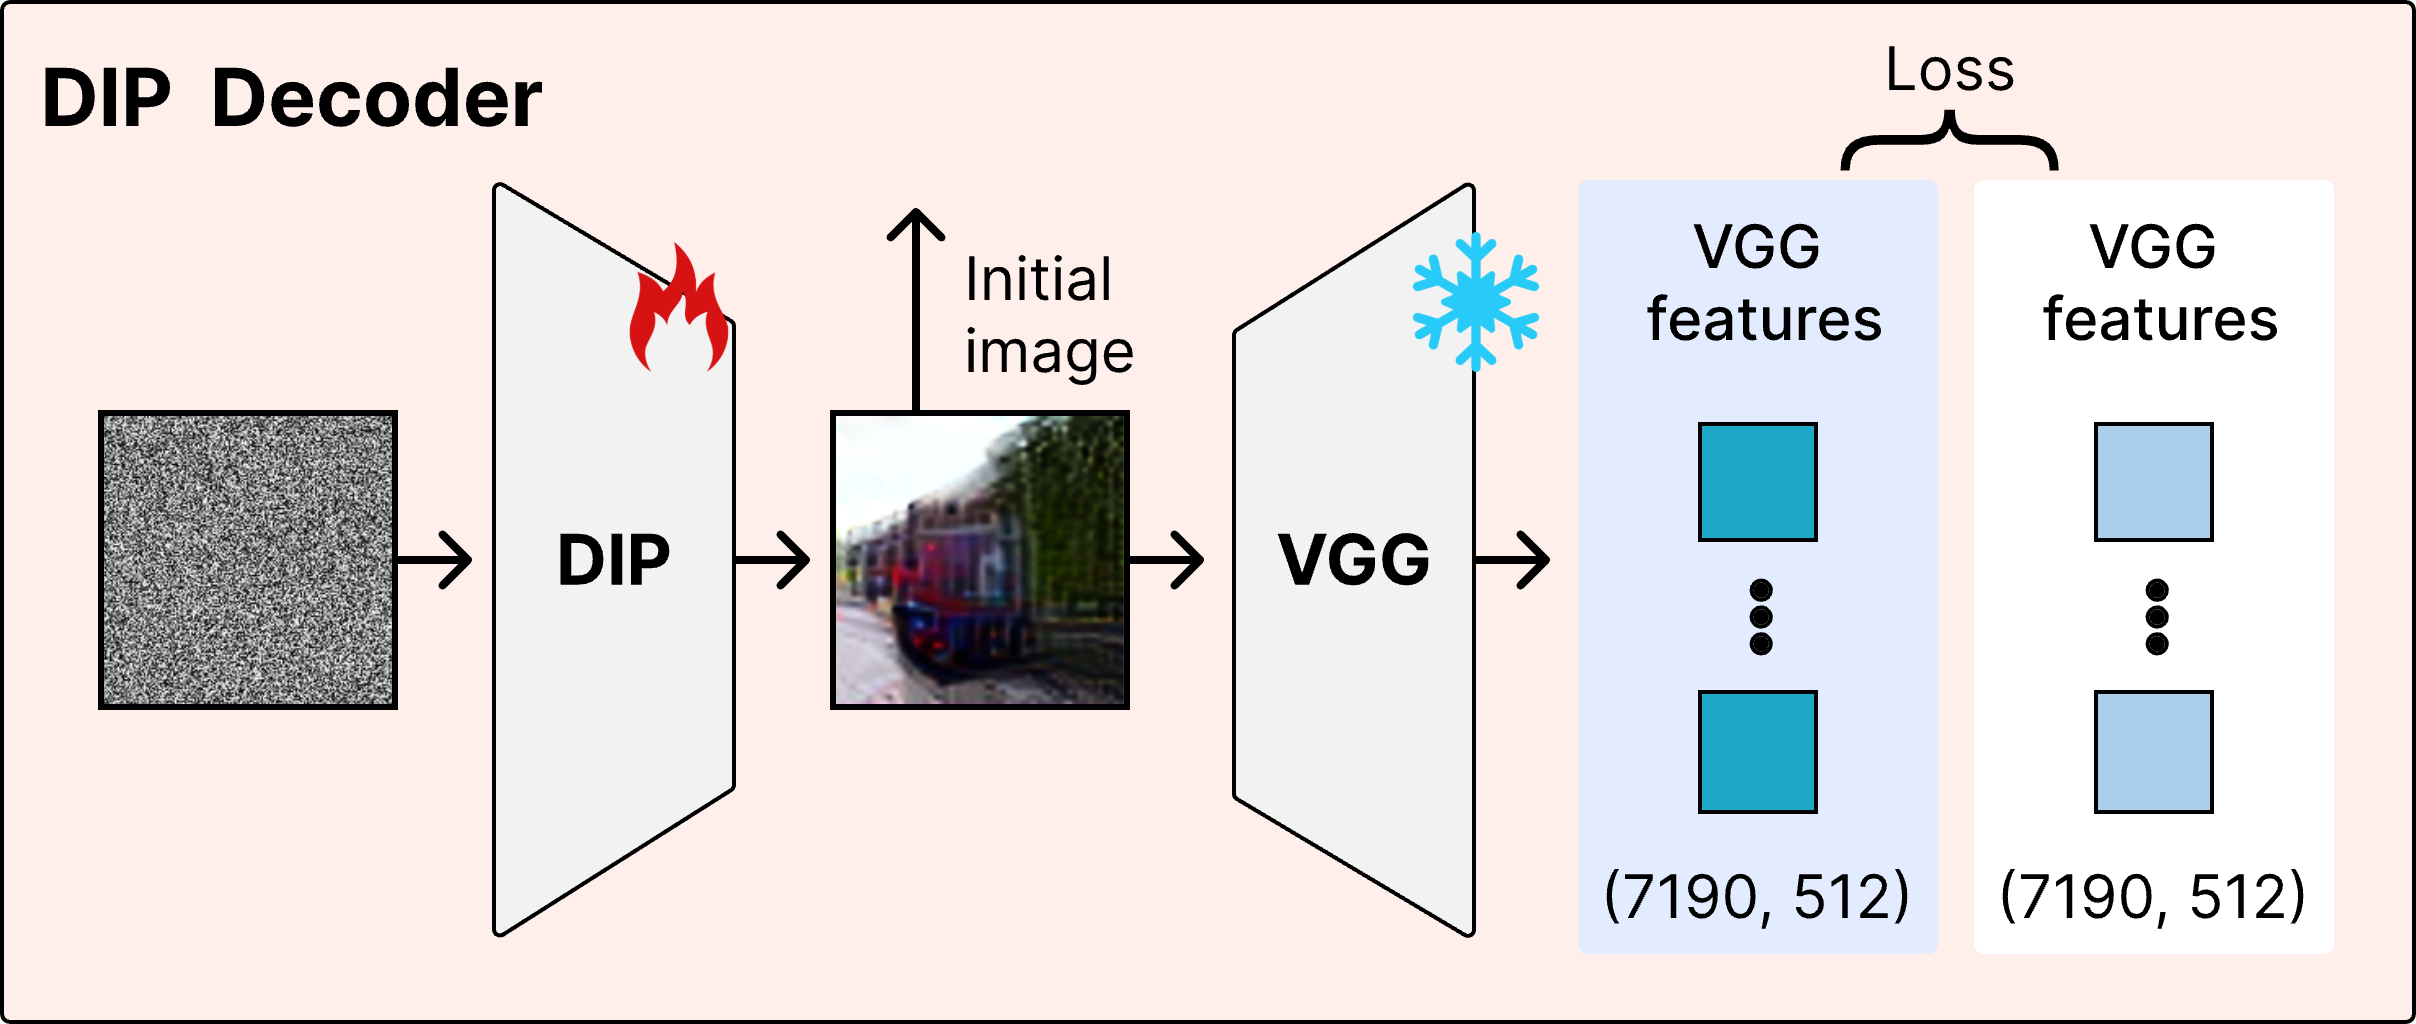
\includegraphics[width=1\columnwidth]{images/DIP3.png}
\caption{Low-level reconstruction with Deep Image Prior. A U-Net maps noise to an image whose frozen VGG16-BN features are matched to the bridge's predicted features. After 2000 optimization steps, its output is the low-level reconstruction.}
\label{fig:dip_reconstruction}
\end{figure}

\subsection{Low-Level Branch}
\label{sec:low_level}
From the predicted VGG feature representation, we reconstruct a low-level image through Deep Image Prior (DIP) inversion. The VGG representation consists of the stacked outputs of five convolutional layers of the VGG16-BN image model.

To convert this representation into the initial image, we optimize a separate DIP U-Net for each image. The U-Net is a small encoder-decoder convolutional generator that maps random Gaussian noise to an RGB image, which is then passed through a frozen VGG16-BN network. The extracted VGG features are compared against the brain-predicted VGG representation using an MSE loss. The gradient is backpropagated only through the DIP U-Net, iteratively updating the generator for a fixed 2000 optimization steps to produce the final low-level reconstruction.

\subsection{Final Image Reconstruction}
To generate the final image reconstruction, we combine the image capturing low-level features generated using DIP with the semantic CLIP prediction using the MindEye2 Stable Diffusion XL unCLIP model (SDXL-unCLIP). SDXL-unCLIP is a pretrained image generation model that generates images from OpenCLIP ViT-bigG/14 image embeddings instead of text-prompt embeddings. The intention is for the low-level DIP image to provide layout, color, and coarse structure while the predicted OpenCLIP ViT-bigG/14 tokens contribute the semantic context of the image.

We first add Gaussian noise to the low-level image to partially corrupt fine detail while preserving coarse layout and color. This re-noised image becomes the initial state for SDXL-unCLIP, anchoring the image structure. The predicted OpenCLIP token representation then steers the denoising process toward the correct semantic context, turning the blurry low-level reconstruction into a detailed final image. With this approach, the reconstruction should reflect both the content and the structure of the stimulus. We run this diffusion process multiple times for each image and select the reconstruction whose downscaled version has the lowest MSE relative to the low-level reconstruction. This keeps the final image from straying too far from the predicted low-level image structure.

\begin{figure}[!t]
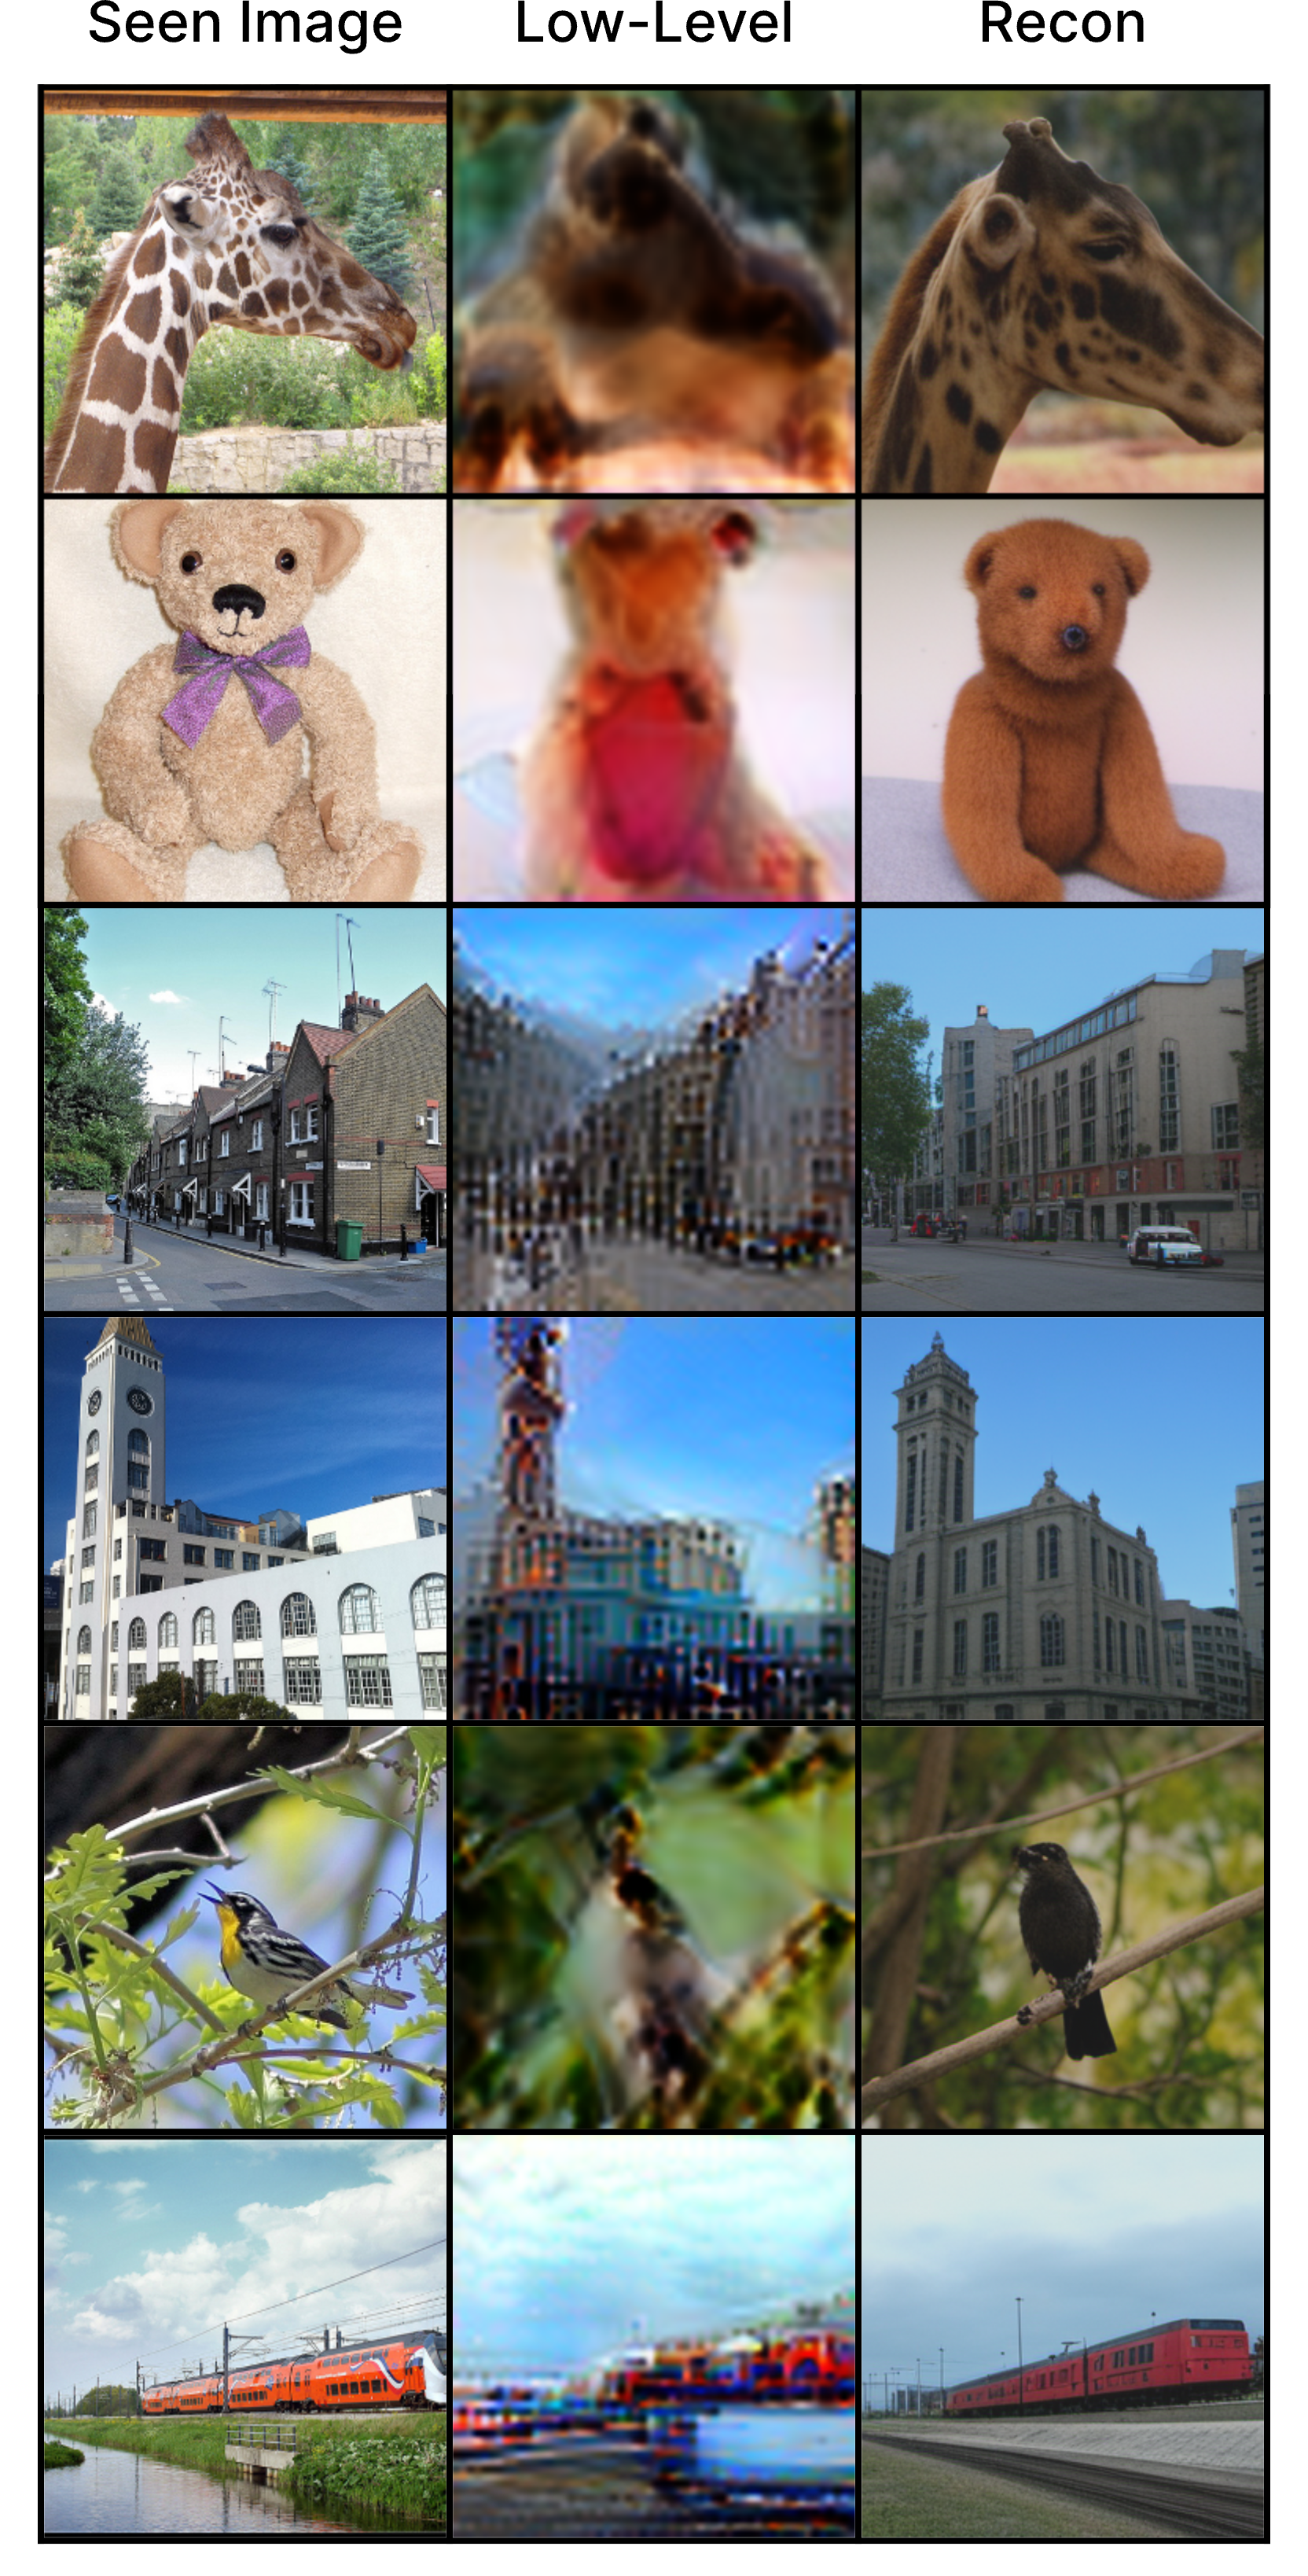
\includegraphics[width=0.65\columnwidth]{images/stacked_triptych_collage3.png}
\centering
\caption{Stimulus (left), low-level DIP reconstruction (middle) and final diffusion reconstruction (right). Images from COCO \cite{lin2015microsoftcococommonobjects} (CC BY 4.0).}
\label{fig:stacked_triptych}
\end{figure}


% You must include your signed IEEE copyright release form when you submit your finished paper.
% We MUST have this form before your paper can be published in the proceedings.

% Please direct any questions to the production editor in charge of these proceedings at the IEEE Computer Society Press:
% \url{https://www.computer.org/about/contact}.
